%% Homework 5 - Tate Mason %%
\documentclass[10pt, a4paper]{article}
\usepackage[top=3cm, bottom=4cm, left=3.5cm, right=3.5cm]{geometry}
\usepackage{amsmath,amsthm,amsfonts,amssymb,amscd, fancyhdr, color, comment, graphicx, environ}
\usepackage{float}
\usepackage{mathtools}
\usepackage{mathrsfs}
\usepackage[math-style=ISO]{unicode-math}
\DeclareSymbolFont{\mathnormal}{letters}
\usepackage{lastpage}

%%%%%%%%%%%%%%%%%%%%%%%%%%%%%%%%%%%%%%%%%%%%%%%%%%%%%%%%%%%%%%%%%%
%%%%%%%%%%%%%%%%%%%%%%%%%%%%%%%%%%%%%%%%%%%%%%%%%%%%%%%%%%%%%%%%%%
%Fill in the appropriate information below
\newcommand{\norm}[1]{\left\lVert#1\right\rVert}     
\newcommand\course{ECON - 8010}                            % <-- course name   
\newcommand\hwnumber{ 5}                                 % <-- homework number
\newcommand\Information{Tate Mason}                        % <-- personal information
%%%%%%%%%%%%%%%%%%%%%%%%%%%%%%%%%%%%%%%%%%%%%%%%%%%%%%%%%%%%%%%%%%
%%%%%%%%%%%%%%%%%%%%%%%%%%%%%%%%%%%%%%%%%%%%%%%%%%%%%%%%%%%%%%%%%%
%Page setup
\pagestyle{fancy}
\headheight 35pt
\lhead{\today}
\rhead{}
\lfoot{}
\pagenumbering{arabic}
\cfoot{\small\thepage}
\rfoot{}
\headsep 1.2em
\renewcommand{\baselinestretch}{1.25}
%%%%%%%%%%%%%%%%%%%%%%%%%%%%%%%%%%%%%%%%%%%%%%%%%%%%%%%%%%%%%%%%%%
%%%%%%%%%%%%%%%%%%%%%%%%%%%%%%%%%%%%%%%%%%%%%%%%%%%%%%%%%%%%%%%%%%
%Add new commands here
\renewcommand{\labelenumi}{\alph{enumi})}
\newcommand{\var}{\text{var}}
\newcommand{\Z}{\mathbb Z}
\newcommand{\R}{\mathbb R}
\newcommand{\Q}{\mathbb Q}
\newcommand{\NN}{\mathbb N}
\newcommand{\PP}{\mathbb P}
\DeclareMathOperator{\Mod}{Mod} 
\renewcommand\lstlistingname{Algorithm}
\renewcommand\lstlistlistingname{Algorithms}
\def\lstlistingautorefname{Alg.}
\newtheorem*{theorem}{Theorem}
\newtheorem*{lemma}{Lemma}
\newtheorem{case}{Case}
\newcommand{\assign}{:=}
\newcommand{\infixiff}{\text{ iff }}
\newcommand{\nobracket}{}
\newcommand{\backassign}{=:}
\newcommand{\tmmathbf}[1]{\ensuremath{\boldsymbol{#1}}}
\newcommand{\tmop}[1]{\ensuremath{\operatorname{#1}}}
\newcommand{\tmtextbf}[1]{\text{{\bfseries{#1}}}}
\newcommand{\tmtextit}[1]{\text{{\itshape{#1}}}}

\newenvironment{itemizedot}{\begin{itemize} \renewcommand{\labelitemi}{$\bullet$}\renewcommand{\labelitemii}{$\bullet$}\renewcommand{\labelitemiii}{$\bullet$}\renewcommand{\labelitemiv}{$\bullet$}}{\end{itemize}}
\catcode`\<=\active \def<{
\fontencoding{T1}\selectfont\symbol{60}\fontencoding{\encodingdefault}}
\catcode`\>=\active \def>{
\fontencoding{T1}\selectfont\symbol{62}\fontencoding{\encodingdefault}}
\catcode`\<=\active \def<{
\fontencoding{T1}\selectfont\symbol{60}\fontencoding{\encodingdefault}}

%%%%%%%%%%%%%%%%%%%%%%%%%%%%%%%%%%%%%%%%%%%%%%%%%%%%%%%%%%%%%%%%%%
%%%%%%%%%%%%%%%%%%%%%%%%%%%%%%%%%%%%%%%%%%%%%%%%%%%%%%%%%%%%%%%%%%
%Begin now!

\begin{document}
  \begin{titlepage}
    \begin{center}
      \vspace*{3cm}
            
        \vspace{1cm}
        \huge
        Homework \hwnumber
            
        \vspace{1.5cm}
        \Large
            
        \textbf{\Information}                      % <-- author
            
        \vfill
        
        An \course \ Homework Assignment
            
        \vspace{1cm}
        \Large

        
        \today
            
    \end{center}
  \end{titlepage}

  \newpage
\section*{PS1 - Question 3}
  \subsection*{Problem}
    In a second-price auction, each of the n bidders simultaneously places a bid for an
    object. The object is won by the bidder with the highest bid, who pays the amount of
    the second-highest bid. If there are multiple highest bids, then the winner is chosen at random from among the highest bidders, and this winner pays the highest bid (since this is also the second-highest bid).

    Suppose that player i values the object at vi dollars, and that all players’ valuations are commonly known. Show that it is a weakly dominant strategy for player i to bid his valuation.
  \subsection*{Solution}
    \begin{proof}
      1. $v_i>x_i$. In this case, player $i$ would win given $u_i(v_i, s_{-i}) > u_i(x_i, s_{-i})$ and $u_i(x_i, s_{-i})$ , or lose if $u_i(x_i, s_{-i}) = 0$ \\
      2. $v_i < x_i$. In this case, player $i$ would win if $u_i(v_i, s_{-i})<u_i(x_i, s_{-i})$ and $u_i(x_i, s_{-i})$ or lose if $u_i(x_i, s_{-i}) = 0$. \\
      3. $v_i = x_i$. In this case, player $i$ would win if $u_i(v_i, s_{-i}) = u_i(x_i, s_{-i})$ and $u_i(x_i, x_{-i}) < 0$ and loses if $u_i(x_i, s_{-i}) = 0$. \\
      Bidding $v_i=x_i$ is a weakly dominated strategy because utility is at least as good as bidding $x_i>v_i$. 
    \end{proof}
\section*{PS1 - Question 4}
  \subsection*{Problem}
    Two travelers returning home from a remote island where they bought identical antiques discover that the airline has managed to smash them. The airline manager decides to use the following scheme to determine the compensation that the airline will give each traveler: Each traveler will separately report the cost of the antique, stating an integer number of dollars between 2 and 500. If both report the same number of dollars, then the airline will give each of them that number of dollars. If they report different numbers of dollars, then the traveler who stated the smaller number will be given the amount he stated plus a bonus of 2 dollars; the traveler who stated the higher number will be given the amount stated by the other traveler minus a penalty of 2 dollars. Suppose that each traveler cares only about maximizing the expected number of dollars he receives from the airline.
    \subsubsection*{(i)}
      Define the normal form game $G$ corresponding to the story above specifying the set of players $\mathcal{P}$, their strategy sets  $S_i$, and their payoff functions $u_i$.
    \subsubsection*{(ii)}
      Fix player 1's beliefs $\mu_1\in\Delta S_2$, and suppose that the highest strategy in $S_2$ that receives positive probability under $\mu_1$ is $\bar{s}_2>2$. Show that player 1's best response given his beliefs must be less than $\bar{s}_2$. (Hint: Start by computing player 1's payoff from choosing a strategy greater than $\bar{s}_2$, and notice that answering the question does not necessarily require you to compute player 1's best response to $\mu_1$)
    \subsubsection*{(iii)}
      If there is a common knowledge of rationality between the players, what is the appropriate prediction of play in $G$?
  \subsection*{Solutions}
    \subsubsection*{(i)}
      \begin{gather*}
        $\mathcal{P} = \{1,2\}$\\
        $S_i \in [2,500]$ \\ 
        \text{Payoffs:}\\
          s_1 = s_2: u(s_1, s_2) = s_i \ for \ i \in [1,2] \\
          s_1 > s_2: u(s_1, s_2) = s_2 - 2 \\
          s_1 < s_2: u(s_1, s_2) = s_1 + 2 \\
      \end{gather*}
    \subsubsection*{(ii)}
      \begin{proof}
        $s_1 > \bar{s}_2$ would result in player 1 receiving payoff $\bar{s}_2-2$. If they were to bid $\bar{s}_2$, the two players would receive equal payoffs. So, by bidding less than $\bar{s}_2$, player 1 will receive their bid + 2 dollars, while the opponent will receive player 1's bid -2 dollars.
      \end{proof}
    \subsubsection*{(iii)}
      \begin{proof}
        Bidding 500 would be dominated by bidding 499. Then, bidding 499 becomes dominated by 498. This iterative elimination process continues until the only option remaining is to bid the minimum, 2 dollars. Thus, under common knowledge, both players bid 2 dollars, receiving an equal payoff.
      \end{proof}
\section*{PS1 - Question 5}
  \subsection*{Problem}
    Consider the following normal form game:
    \begin{center}
      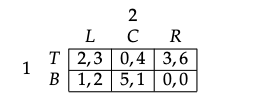
\includegraphics[width = 0.4\textwidth]{PS1-5.png}
    \end{center}
    \subsubsection*{(i)}
      Are any pure strategies in this game strictly dominated? If so, then for each such strategy $s_i$, identify all dominating strategies that do not put positive probability on $s_i$.
    \subsubsection*{(ii)}
      If there is common knowledge of rationality between the players, what should our prediction of play in this game be?
  \subsection*{Solutions}
    \subsubsection*{(i)}
      No matter $P_1$'s strategy, $P_2$ will never choose the center column. Thus, a mixed strategy of L and R exist which strictly dominate C. \\
      $P_1$ chooses T: 
      \begin{gather*}
        3P + (1-P)6 > 4 \\
        6 - 3P > 4 \\
        3P < 2 \\
        P < \frac{2}{3} 
      \end{gather*}
      $P_1$ chooses B:
      \begin{gather*}
        2P + (1-P)0 > 1 \\
        2P > 1 \\
        P > \frac{1}{2}
      \end{gather*}
      So, a strategy of choosing L with probability $\frac{1}{2} < P < \frac{2}{3}$ and R with probability $(1-p)$ strictly dominates. 
    \subsubsection*{(ii)}
      Common knowledge will see strategy $(T,R)$ chosen. 
\section*{PS1 - Question 7}
  \subsection*{Problem}
    Which pure strategies are rationalizable in the following normal form game? Explain.
    \begin{center}
      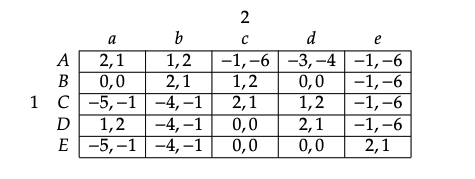
\includegraphics[width = 0.72\textwidth]{PS1-7.png}
    \end{center}
  \subsection*{Solution}
    All pure strategies for both players are rationalizable.
\section*{PS2 - Question 1}
  \subsection*{Problem}
    Compute all Nash equilibria in the following game:
    \begin{center}
      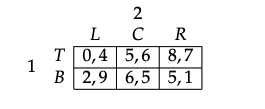
\includegraphics[width = 0.4\textwidth]{PS2-1.png}
    \end{center}
  \subsection*{Solution}
    $\{(T,R), (B,L)\}$ are pure strategy Nash equilibria. \\
    C is not a pure strategy, so we should look for mixed strategy of L and R which strictly dominates pure strategy C.
    $P_1$ chooses T:
    \begin{gather*}
      $4p + (1-p)7 > 6$ \\
      $7 - 3P > 6$ \\
      $3P < 1$ \\
      $P < \frac{1}{3}$
    \end{gather*}
    $P_1$ chooses B:
    \begin{gather*}
      $9P + (1-P)1 > 5$ \\
      $8P > 4$ \\
      $P > \frac{1}{2}$
    \end{gather*}
    This probability of a mixed strategy is not feasible, so we can infer that $P_2$ is at least indifferent between two strategies. So when $P_1$ mixes their strategies:
    \begin{gather*}
      U_2(L,\sigma_1) = 4P + (1-P)9 = 9 - 5P \\
      U_2(C, \sigma_1) = 6P + (1-P)5 = 5 + P \\
      U_2(R, \sigma_1) = 7P + (1-P)1 = 1 + 6P \\
      \\
      9-5P = 5 + P \rightarrow 4 = 6P \rightarrow P = \frac{2}{3} \\
      9-5P = 1 + 6P \rightarrow 8 = 11P \rightarrow P = \frac{8}{11} \\
      5+P = 1 + 6P \rightarrow 4 = 5P \rightarrow P = \frac{4}{5}
    \end{gather*}
    If $U_2(R, \sigma_1)=U_2(C, \sigma_1)$, $P = \frac{4}{5}$ and $U_1(T,\sigma_2) = U_1(B,\sigma_2)$, giving us the following:
    \begin{gather*}
      5P + (1-P)8 = 6P + (1-P)5 \\
      8 - 3P = 5 + P \\
      3 = 4P \\
      P = \frac{3}{4} \\
    \end{gather*}
    Thus, we can see mixed strategy Nash is $(\frac{4}{5}T + \frac{1}{5}B, \frac{3}{4}C + \frac{1}{4}R)$. \\
    \\
    In conclusion, the full list of Nash equilibria is $\{(T,R), (B,L), (\frac{4}{5}T + \frac{1}{5}B, \frac{3}{4}C + \frac{1}{4}R)\}$.
\section*{PS2 - Question 2} 
  \subsection*{Problem}
    Find all Nash equilibria in the following game: 
    \begin{center}
      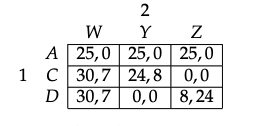
\includegraphics[width=0.4\textwidth]{PS2-2.png}
    \end{center}
  \subsection*{Solution}
    Pure Nash equilibria are $\{(A, Y), (A, Z)\}$. The mixed strategy is calculated as following:
    \begin{gather*}
      \sigma_1 = \{C,D\} \\
      U_2(W, \sigma_1) = 7P + (1-P)7 = 7 \\
      U_2(Y, \sigma_1) = 8P + (1-P)0 = 8P \\
      U_2(Z, \sigma_1) = 0P + (1-P)24 = 24 - 24P \\
      \\
      7 = 8P \rightarrow P = \frac{7}{8} \\
      7 = 24 - 24P \rightarrow P = \frac{17}{24} \\
      8P = 24 - 24P \rightarrow 32P = 24 \rightarrow P = \frac{3}{4} \\
      \\
      U_2(Y, \sigma_1) = U_2(Z, \sigma_1) = \frac{3}{4}\\
      U_1(C, \sigma_2) = U_1(D, \sigma_2): \\
      \\
      24P + (1-P)0 = 0P + (1-P)8 \\
      24P = 8 - 8P \\
      32P = 8 \\
      P = \frac{1}{4}
    \end{gather*}
    So, there is also mixed strategy Nash equilibrium $(\frac{3}{4}C + \frac{1}{4}D, \frac{1}{4}Y + \frac{3}{4}Z)$. \\
    \\
    In conclusion, all Nash equilibria are $\{(A,Y), (A,Z), (\frac{3}{4}C + \frac{1}{4}D, \frac{1}{4}Y + \frac{3}{4}Z)\}$.
\end{document}

